%% LaTeX2e class for student theses
%% sections/methodology.tex
%% 
%% Karlsruhe Institute of Technology
%% Institute for Program Structures and Data Organization
%% Chair for Software Design and Quality (SDQ)
%%
%% Dr.-Ing. Erik Burger
%% burger@kit.edu
%%
%% Version 1.3.6, 2022-09-28

\chapter{Methodology}
\label{ch:Methodolody}

%% -------------------
%% | Example content |
%% -------------------
Since our continual active learning approach is, to the best of our knowledge, the first approach to combine pool-based active learning with continual
learning, we explain it in detail in this chapter, including its motivation. We then transfer our approach to the model stealing domain. Because we
build upon the framework of ActiveThief, we describe how our method compares to the original one in detail.

\section{Continual Active Learning}
\label{sec:Methodology:ContinualActiveLearning}
The main contribution of this thesis is combining the two learning paradigms continual learning and active learning. To motivate the idea of combining
these two paradigms, we will first outline the classic continual learning setting and the classic active learning setting.
Next, we explain common issues with these two learning paradigms and how we aim to overcome these by combining both paradigms. Finally, we describe a custom
Replay strategy, which we use in our experiments.

\subsection{Classic Continual Learning Setting}
\label{sec:Methodology:CLSetting}
In the typical continual learning setting, the model is trained on a sequence of tasks. Each task $T_i = \{(x_k,y_k) | k \in \{1,\ldots,n\}\}$ is a set
of instances with their respective label. Together, the tasks form a dataset $D = \bigcup\limits_{i=1}^{N} T_i$. Note that
the distributions of two distinct tasks $P(T_i)$  and $P(T_j) (i \neq j)$ are not necessarily the same. Often the tasks are independent, which is why
neural networks struggle to perform well on multiple tasks simultaneously. This also means that the size of two distinct datasets
can be different, i.e., $|T_i| \neq |T_j|$ and so can the number of classes $|\{y_k | \exists x_k: (x_k,y_k) \in T_i \}| \neq |\{y_l | \exists x_l: (x_l,y_l)
\in T_j\}|$. When training a model on a sequence of tasks, the model is first fed with the data of the first task $T_1$ and then trained on it. 
After the model was trained on the first task, it can either be trained on the next task or deployed to classify samples stemming from the
distribution of the first task. Next, the model is trained on the second task. After being trained on the second task, the model should now be able to
classify samples from the distribution of the first and second tasks. This process repeats until the model has been trained on all
tasks. At the end of the process, the model should be able to classify samples following the distribution of all the tasks it was trained on.
This workflow is illustrated in figure \ref{fig:CLWorkflow}. \par
The main difference between the continual learning setting and classic machine learning is that in the classic machine learning setting, the model is
not retrained after deployment. In the continual learning setting, however, the model is retrained whenever a new task arrives.

\begin{figure}[ht]
    \centering
    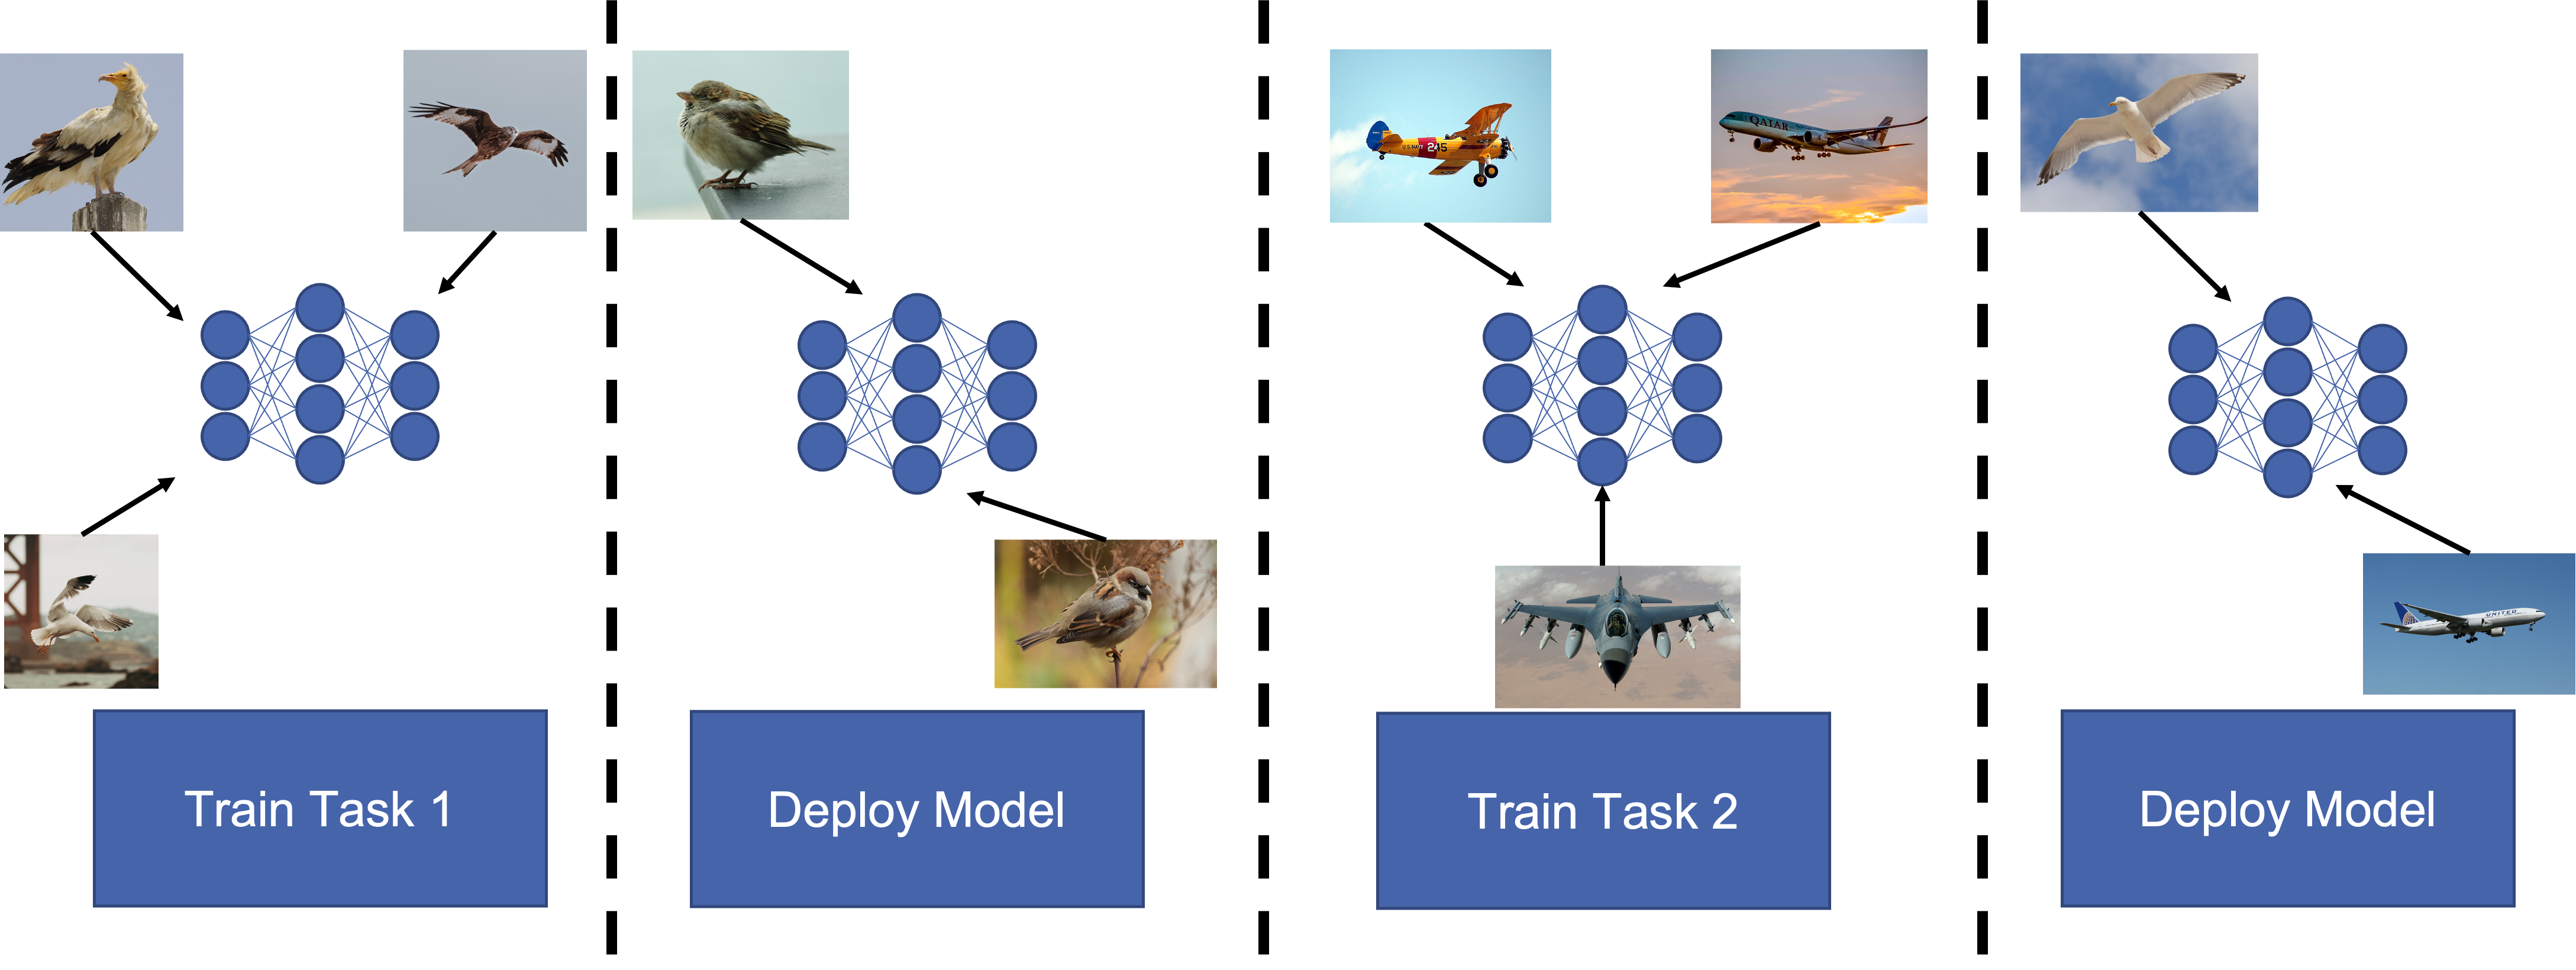
\includegraphics[width=.9\linewidth]{images/CL_workflow.png}
    \caption[Continual learning workflow]{Example for the classic continual learning workflow. In this example, the model is first trained on different species of
    birds. It is then deployed to differentiate these species. Next, the model is trained on planes. After being deployed again, the model should now differentiate
    the planes as well as the birds.}
    \label{fig:CLWorkflow}
  \end{figure}

\subsection{Pool-based Active Learning Setting}
\label{sec:Methodology:ALSetting}
In the pool-based active learning setting, the model is trained sequentially on the current labeled pool. At first, the labeled pool is empty. Next, it is
initialized by randomly selecting samples from the unlabeled pool to label. On the contrary, the unlabeled pool contains the complete dataset at first and
is emptied in the process. After initializing the labeled pool, the model is trained on it. Next, $b$ samples from the labeled pool are selected until the
total budget is exhausted. The selected samples are the ones determined to be the most informative by the current active learning strategy. The oracle labels
them, and then they added to the labeled pool. Next, the model is trained on the current labeled pool, and the process repeats. We provide a more detailed
description of pool-based active learning in section \ref{sec:PoolBasedActiveLearning}. \par
Active learning contrasts with continual learning because all data stems from the same task. Another difference between pool-based active learning and
continual learning is that a model trained by active learning is trained on all previously selected batches. Consequently, the model is trained on some
data multiple times, which might cause parts of the training to be redundant.

\subsection{Combining Continual and Active Learning}
\label{sec:Methodology:CombiningCLandAL}
The problem with classic active learning is that it is very resource intensive. When training a model using pool-based active learning on a dataset of size $n$,
with batch size $b$, the model will be trained $\frac{n}{b}$ times on the current labeled pool, equating to $\frac{n(n+b)}{2b}$ data points overall (we provide a
short derivation of this formula in \ref{sec:appendix:FirstSection}). The problem with the number of data points used for training is that it is dependent on the
batch size $b$. The smaller the batch size, the larger the overall number of data points that the model is trained on. In the extreme case of $b=1$, the model
is trained on $\frac{n(n+1)}{2}$ data points. While \cite{beck2021effective} note that the batch size has a negligible effect on the model performance, a typical
batch size is less than ten percent of the complete training set. Even in this more realistic case, the model is trained on $5.5n$ data points. When
comparing this to the classic continual learning setting, where the model is trained once using $n$ data points, it is clear that active learning comes with
considerable overhead. The overhead of active learning is even more pronounced when considering the execution time of the active learning algorithms.
For more details, we refer to chapter \ref{ch:Evaluation} and \ref{ch:Discussion}. \par
On the other hand, a massive problem with classic continual learning is that task order significantly impacts the model performance \cite{bell2022effect}.
Hacohen et al. studied the problem of task ordering previously and showed that training samples in decreasing order of difficulty results in faster learning and
improved generalization error \cite{hacohen2019power}. This motivates us to use active learning to perform task ordering. We should note here that we
assume the free choice of the next task. This assumption is not always realistic, especially when tasks arrive sequentially, but studying the effect of task-ordering
benefits the study of these scenarios, too. Furthermore, insights into task-ordering help towards a more rigorous evaluation of continual learning in 
research because they allow us to assess the influence of task-ordering on experiment results when using classic benchmark datasets. \par
Our approach aims to overcome the overhead of active learning and the issue of task ordering by combining both learning paradigms. We modify the active
learning process by training only on the currently selected batch instead of the entire labeled pool. This way, the model is trained on $\sum_{i=1}^{\frac{n}{b}} b = n$ 
data points, which fully eliminates the overhead of active learning from a data-centric perspective. Nevertheless, the query time of the active learning algorithm remains
an overhead. From a continual learning perspective, we join all tasks to a single dataset and use this dataset as the unlabeled pool for active learning. In each iteration
of the active learning process, we select a batch $B$ from the unlabeled pool using the given active learning strategy. Next, the oracle labels this batch.
We then treat the current batch $B$ as a new task and train our model using only the data points of $B$ with the continual learning strategy of
choice. This process repeats until the unlabeled pool is empty. The full algorithm is described in algorithm \ref{alg:PoolBasedContinualActiveLearning}, where we highlight
the difference between classic pool-based active learning and our new continual active learning approach in bold. \par

\begin{algorithm}
    \caption{Pool-based continual active learning} \label{alg:PoolBasedContinualActiveLearning}
    \begin{algorithmic}[1]
        \Require Unlabeled data $U$, Labeled data $L = \emptyset$, Oracle $O$, Model $M$, budget $B$
        \State Select $k$ data points from $U$ at random, obtain labels by querying $O$ and set $L=\{x_1,\ldots,x_1\}$
        and $U = U \setminus \{x_1,\ldots,x_1\}$ \Comment{Initialization}
        \State Train $M$ on initial labeled set $L$
        \While{Label budget $B$ not exhausted}
            \State Select $l$ data points from $U$ predicted to be the most informative by the active learning strategy
            \State Obtain labels $y_i,\ldots,y_l$ by querying $O$ for $x_i,\ldots,x_l$
            \State \textbf{Train $M$ on current labeled batch $\{\mathbf{(x_i,y_i),\ldots,(x_l,y_l)}\}$}
            \State Set $L= L \cup \{x_i,\ldots,x_l\}$ and $U = U \setminus \{x_i,\ldots,x_l\}$
        \EndWhile
    \end{algorithmic}
\end{algorithm}

\subsection{Replay strategy}
\label{sec:Methodology:ReplayStrategy}
In this subsection, we describe a continual learning strategy named Replay. Applying Replay to overcome catastrophic forgetting is not an entirely new idea.
On the contrary, Robins et al. first proposed using Replay in the 1990s \cite{robins1995catastrophic}. The approach we describe modifies the classic Replay
by compressing the replay buffer. To understand the modification, we must first understand the classic Replay strategy. \par
Replay is a continual learning strategy that stores a subset (or all) data points from each task in a so-called replay buffer. When training on a new task
$T_N$, the model is trained on the data from the current task plus a sample from the replay buffer. After training on task $T_N$, the replay buffer is updated
with the data points from the current task. \par
A significant drawback of the classic Replay strategy is that the replay buffer can grow to extreme sizes over time. This is especially true when the replay
buffer stores all data points from each task. It is more desirable to have a continual learning strategy with a fixed memory footprint because this reflects
real-world applications of continual learning where memory is limited. \par
Our proposed modification of the Replay strategy is to compress the replay buffer after each task. Assume we have a replay buffer of size $n$. After
training on task $T_N$, the replay buffer is combined with the data points from the current task to form a new set of data points $P$. We then select $n$
data points from $P$ to create the new replay buffer. These points are selected by performing one iteration of the active learning strategy CoreSet
\cite{sener2017active} with $P$ as the unlabeled pool and $n$ as the batch size. The $n$ data points selected by CoreSet then represents the new replay buffer.
When training on task $T_{N+1}$, the model is trained on the data from the current task plus the full replay buffer.

\section{Continual Active Learning for Model Stealing}
\label{sec:Methodolody:CALMS}
In this section, we describe how we apply the continual active learning approach to model stealing. Using the continual active learning approach
in the model stealing domain allows us to determine if continual active learning achieves similar performance in the model stealing domain compared to
the standard setup where the oracle returns truthful labels. We motivate transferring our approach to the model stealing domain by highlighting the
 differences between the setup mentioned in \ref{sec:Methodology:CombiningCLandAL} and continual active learning for model stealing. \par
The first difference is that the labels returned by the oracle in the model stealing domain have a limited semantic meaning. This is because the oracle
 is another machine learning model. So even if the data point whose label is queried stems from the same distribution as the target model dataset,
the label returned by the oracle is not necessarily correct since machine learning models do not generalize perfectly. Since the target model dataset
is unknown to the attacker, he cannot knowingly construct a thief dataset that overlaps with the target model dataset. Therefore, the data points the
 attacker queries the target model with will most likely be from a different distribution than the target model dataset and the labels returned by the target model
will be incorrect. The example in figure \ref{fig:CalmsWorkflow} highlights the meaning of the associated label. In the given example, the target model 
is trained to classify planes, which is why it associates the label \enquote{Fighter Jet} with a sparrow. \par
The second difference between the standard continual active learning approach and continual active learning for model stealing lies again in the labels
returned by the oracle. In the classic continual active learning approach, the labels of the oracle are not only truthful, but the label is just a
single value, i.e., the respective class. In the model stealing domain, the label returned by the oracle is either a single value or the per-class
probabilities of the output layer of the target model. The latter is the more interesting case for continual active learning because it reveals more
information about the function learned by the target model. \par
Next, we describe how we apply continual active learning for model stealing. The first step is to use the thief dataset as the initial unlabeled pool for
active learning. The active learning strategy uses the thief dataset in each iteration, just as in classic continual active learning. After selecting the
most informative samples to label, the target model is queried for the labels of the selected samples. Next, the label returned, which is either a single
value or the per-class probabilities of the output layer of the target model, is used as the label of the respective data point throughout the complete
training process. This means that the gradient updates during training are based on the loss computed with a softmax label, allowing for a more fine-grained
optimization of the weights to approximate the target model function. This
process is repeated until the unlabeled pool is empty. A visual example of continual active learning for model stealing is shown in figure
\ref{fig:CalmsWorkflow}. \par
\begin{figure}[ht]
    \centering
    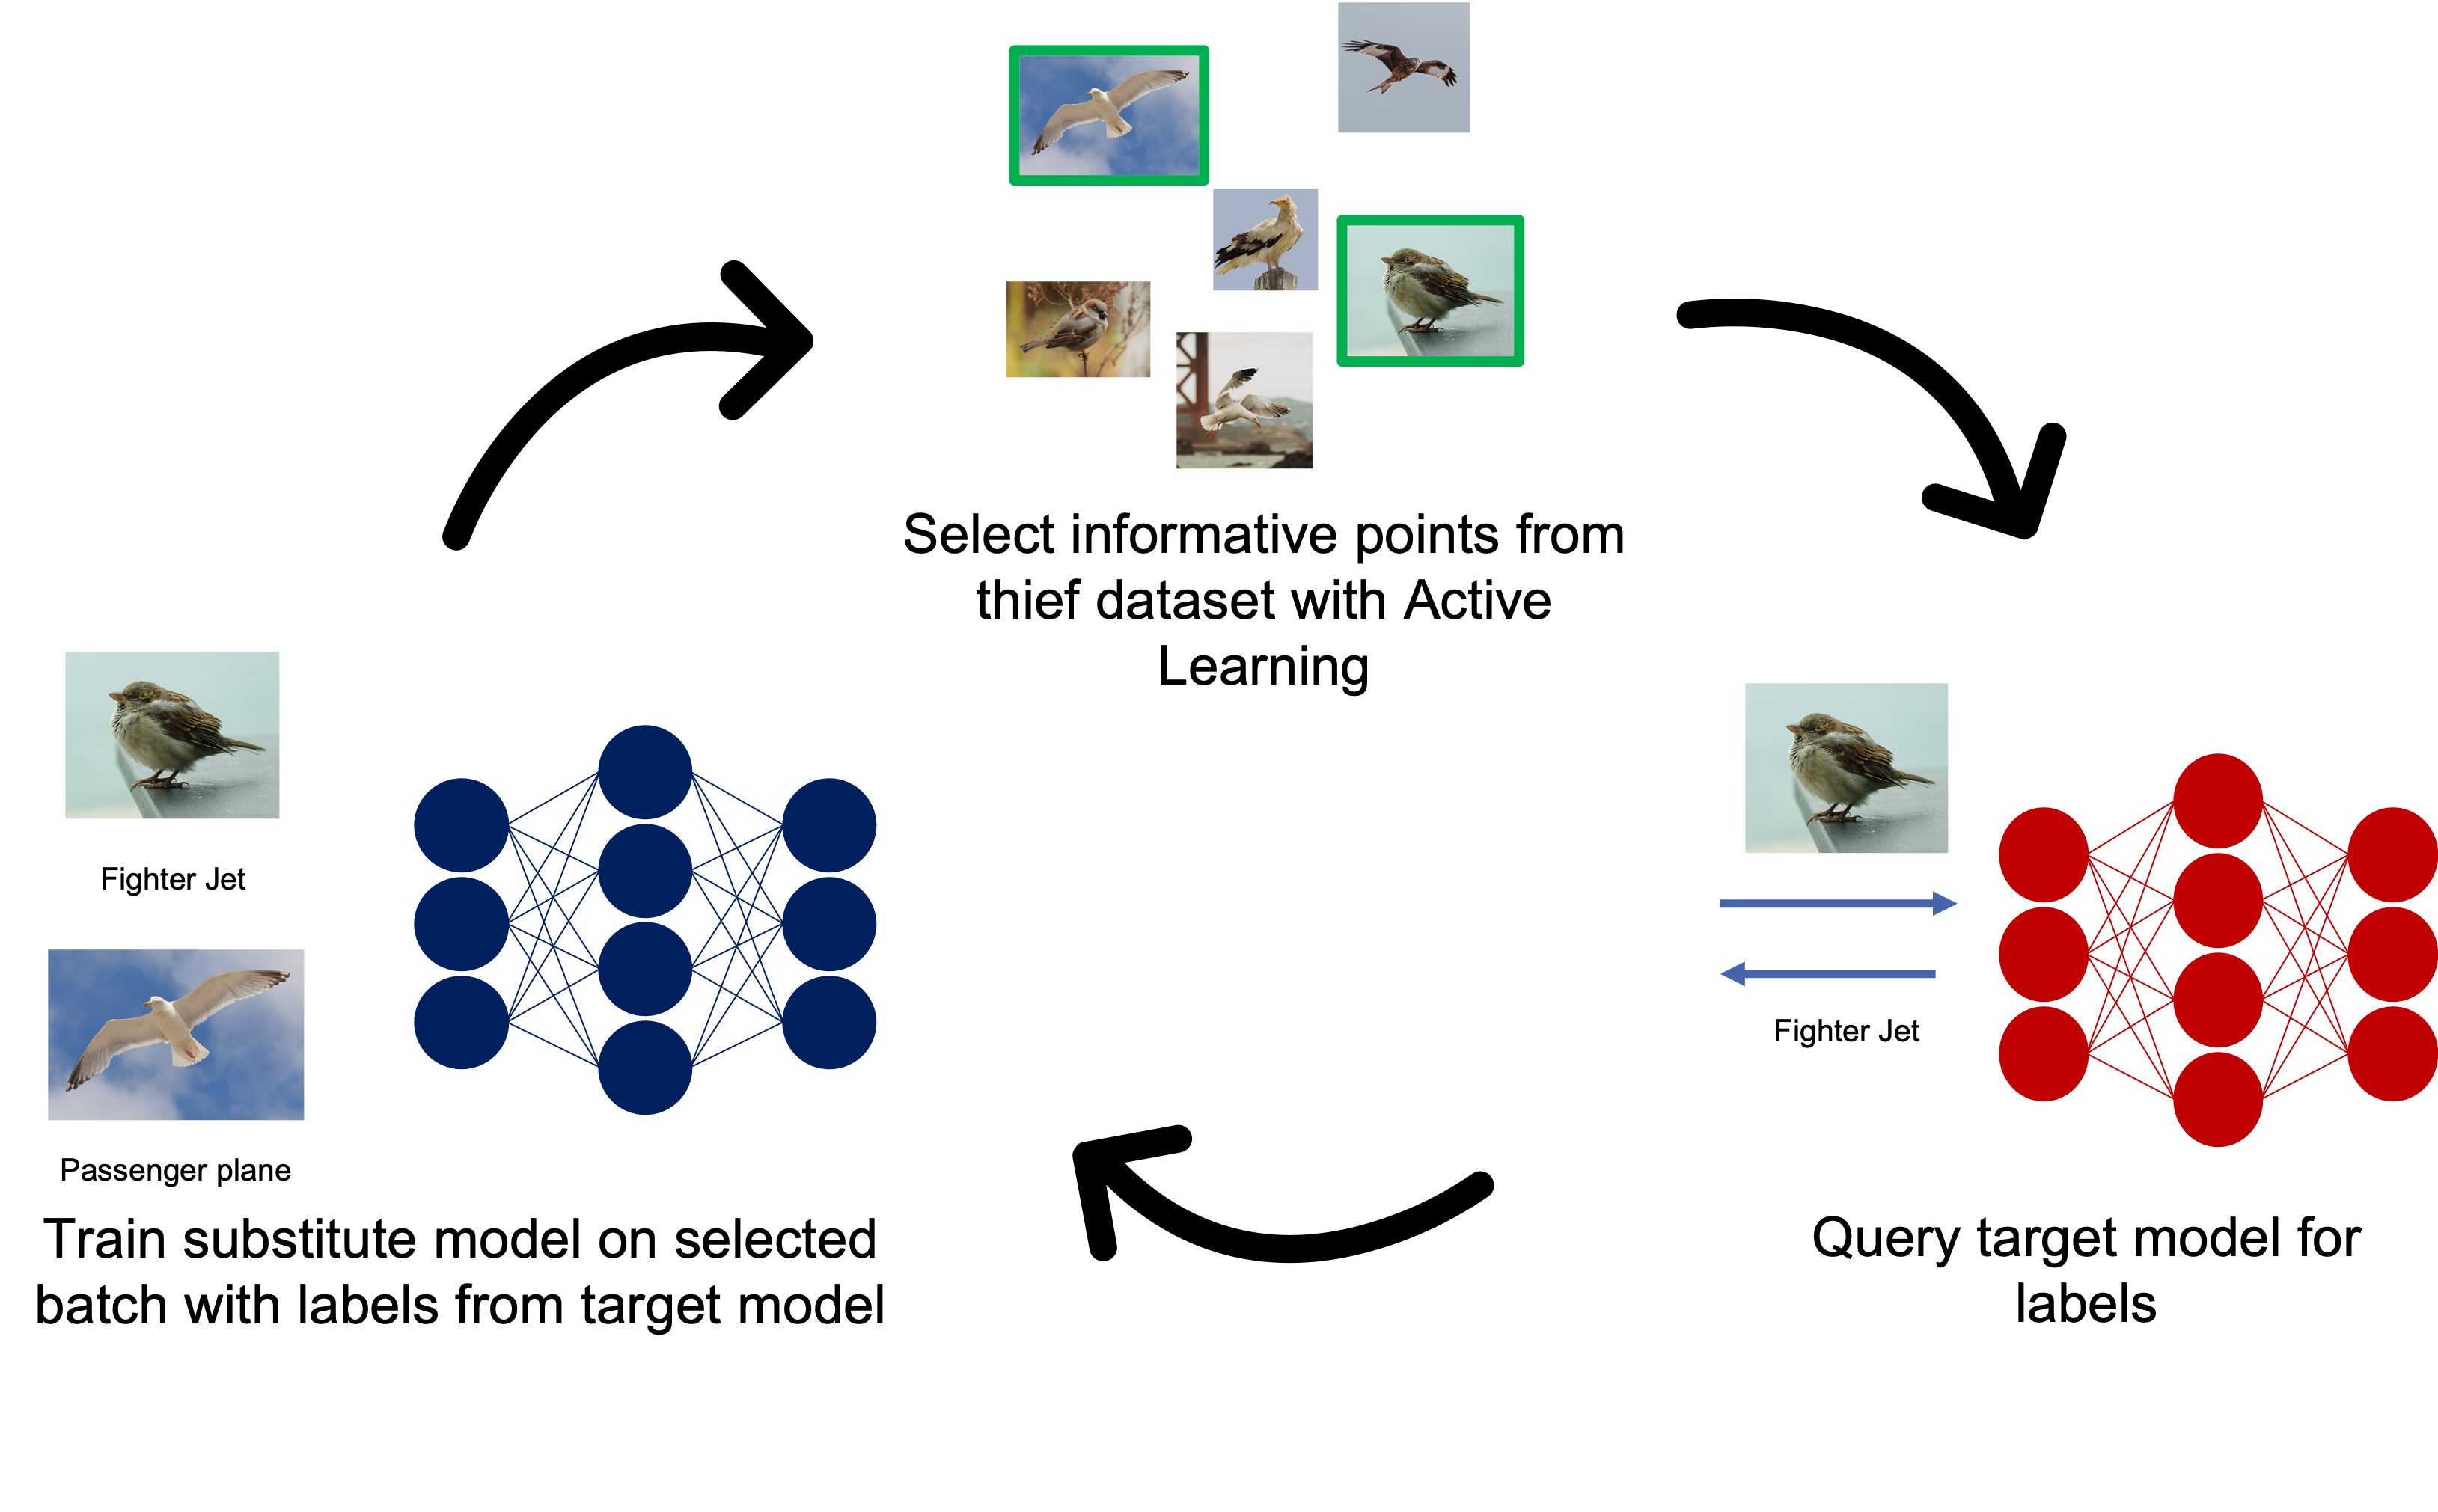
\includegraphics[width=.7\linewidth]{images/Calms_workflow.png}
    \caption[Continual active learning for model stealing example]{Example of continual active learning for model stealing. In this example, the thief
    dataset consists of birds, while the target model was trained to classify planes. In each iteration, a batch of informative samples is selected by the active learning
    strategy. Next, the target model is queried for the labels of the selected samples. Since our thief dataset is composed of \gls{nnpd} data, the associated labels have
    an incorrect semantic meaning. The thief model is then trained on the selected samples from the current batch. This process is repeated iteratively.}
    \label{fig:CalmsWorkflow}
\end{figure}



%% ---------------------
%% | / Example content |
%% ---------------------